\subsection{Validazione}
\subsubsection{Scopo}
Lo scopo di questa sezione è fissare come il gruppo ha deciso di attuare il processo di \glo{validazione}. Questo comprende le attività di controllo mirate a confrontare che il prodotto sia conforme ai requisiti accordati con il \glo{proponente}.

\subsubsection{Aspettative}
\begin{itemize}
	\item Dimostrare la correttezza delle attività svolte in fase di verifica; 
	\item Avere la certezza che il prodotto software rispetti i requisiti riportati nell'\AdRv{v4.0.0-1.8}.
\end{itemize}

\subsubsection{Descrizione}
Il processo di validazione accerta che il prodotto realizzato sia conforme alle attese del \glo{proponente}. Questo processo viene eseguito successivamente al processo di verifica, in modo che tutte le unità del sistema permettano un test completo su di esso.
\subsubsection{Istanziazione del processo}


\paragraph{Procedimento di validazione della documentazione}

%Di seguito viene mostrato il diagramma delle attività esplicativo del processo di validazione da applicare a tutti i documenti prodotti dal gruppo \Gruppo{} durante il progetto.

\begin{figure}[!htb]
     \centering
     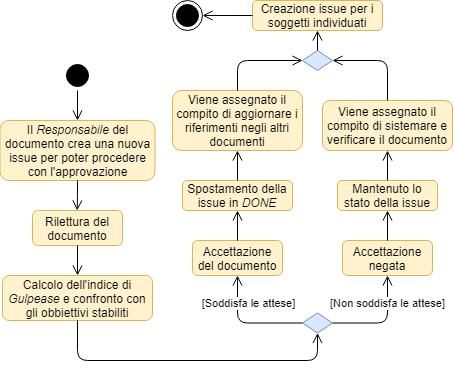
\includegraphics[scale=0.75]{Images/valDocs.png}
     \caption{Diagramma delle attività di validazione della documentazione}
\end{figure}


\paragraph{Procedimento di validazione del codice}

%Di seguito viene mostrato il diagramma delle attività esplicativo del processo di validazione da applicare a tutti i documenti prodotti dal gruppo \Gruppo{} durante il progetto.

\begin{figure}[!htb]
     \centering
     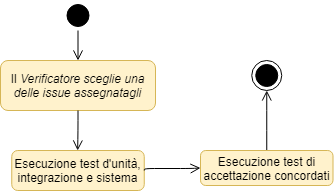
\includegraphics[scale=0.8]{Images/valCode.png}
     \caption{Diagramma delle attività di validazione del codice}
\end{figure}

\paragraph{Test}
In questa fase vengono eseguiti i test di accettazione. Le specifiche dei test vengono illustrate in forma tabellare, contenente il codice del test, la descrizione e il suo stato:
	\begin{itemize}
		\item \textbf{I}: Il test è stato implementato;
		\item \textbf{NI}: Il test non è stato implementato;
		\item \textbf{S}: Il test è passato con successo;
		\item \textbf{F}: Il test è fallito.
	\end{itemize}	 

\mbox{}

\textbf{Test di accettazione}\\
Ogni test di accettazione è identificato da il seguente codice:
\begin{center}
\textbf{TA[ImportanzaRequisito]*[TipologiaRequisito]*[IdNumerico]} 
\end{center}
Singolarmente essi rappresentano:
\begin{itemize}
	\item \textbf{ImportanzaRequisito \& TipologiaRequisito}: questi campi identificano il requisito che si vuole testare (o più requisiti con la stessa importanza e stessa tipologia), seguendo ciò che è riportato al paragrafo \ref{para:requisiti};
	\item \textbf{IdNumerico}: codice numerico crescente che parte da 1.
\end{itemize}


\subsubsection{Metriche}
Il processo di validazione non fa uso di metriche qualitative particolari.

\subsubsection{Strumenti}
Non sono stati identificati degli strumenti particolari per la validazione.

